\subsection{A*}
\label{subsec:a-star-subsection}

Алгоритм A* --- це широко використовуваний алгоритм пошуку шляху, який є розширенням алгоритму Дейкстри. Як і алгоритм Дейкстри, A* використовує евристичну функцію для спрямування пошуку до цільової вершини, але він також враховує вартість вже пройденого шляху. Це дозволяє йому здійснювати пошук більш ефективно, досліджуючи спочатку найбільш перспективні шляхи.

Алгоритм A* працює, підтримуючи два списки: відкритий і закритий. Відкритий список містить вузли, які були відвідані, але ще не розширені, тоді як закритий список містить вузли, які вже були розширені. Спочатку у відкритому списку знаходиться лише початкова вершина. Потім алгоритм багаторазово вибирає вершину з найменшим значенням f (де f(n) = g(n) + h(n), де g(n) - вартість шляху від початкової вершини до вершини n, а h(n) - евристична оцінка вартості шляху від вершини n до мети) і розширює її, додаючи до відкритого списку її сусідів, якщо вони ще не були відвідані.

Алгоритм A* продовжує роботу до тих пір, поки цільова вершина не буде обрана для розширення або поки відкритий список не стане порожнім (в цьому випадку не буде шляху до цільової вершини). Як тільки цільовий вузол досягнуто, алгоритм відстежує шлях назад, слідуючи за вказівниками від цільового вузла до початкового вузла.

Основною перевагою алгоритму A* є його здатність ефективно шукати, використовуючи як вартість вже пройденого шляху, так і евристичну оцінку вартості, що залишилася. Це дозволяє йому знаходити найкоротший шлях швидше, ніж алгоритм Дейкстри. Крім того, A* можна легко налаштувати, змінивши евристичну функцію відповідно до конкретної задачі, що розв'язується.

Однак алгоритм A* також має деякі недоліки. По-перше, він вимагає евристичної функції, яка є одночасно допустимою (ніколи не переоцінює справжню вартість для цільової вершини) і несуперечливою (задовольняє нерівності трикутника). Пошук відповідної евристичної функції може бути складним завданням, особливо для складних задач. По-друге, A* не завжди може знайти оптимальний шлях, якщо евристична функція підібрана невдало. Нарешті, продуктивність A* може бути чутливою до вибору структур даних, що використовуються для зберігання відкритих і закритих списків, а також до деталей реалізації алгоритму.\\

\begin{figure}[!htp]
    \centering
    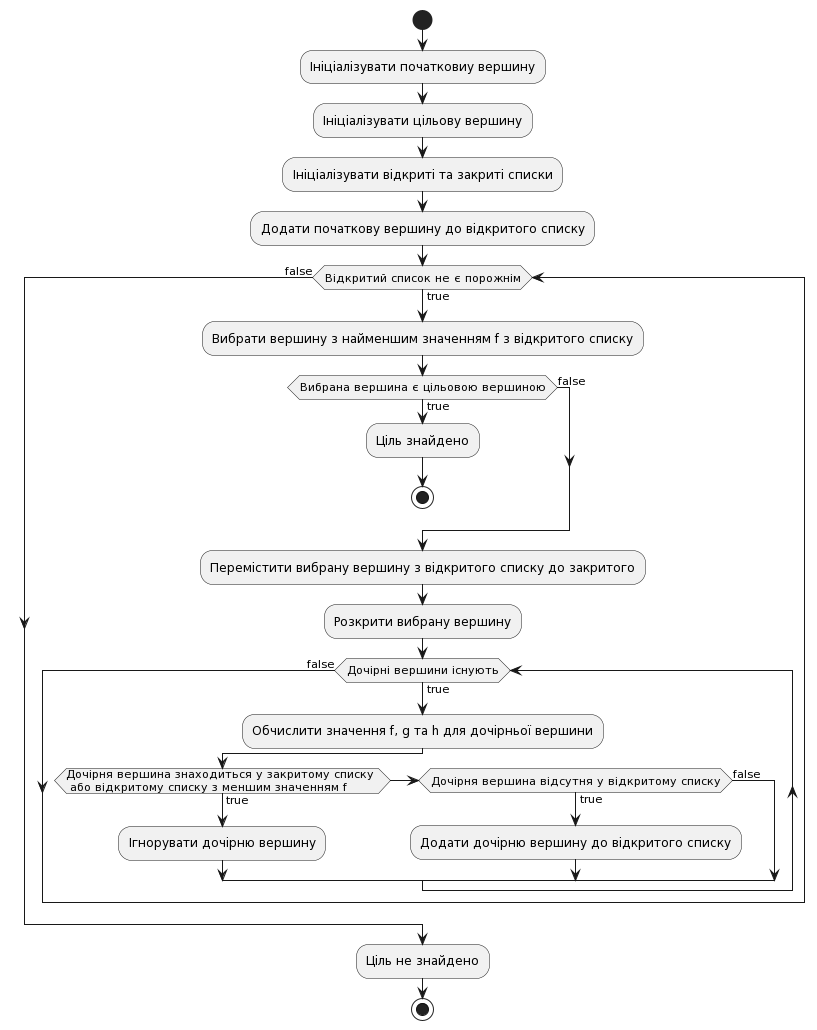
\includegraphics[scale=0.5]{content/chapters/2-implementation-methods/assets/img/a_star_algorithm.png}
    \caption{Блок-схема алгоритму A*}
    \label{fig:a-star}
\end{figure}

Переваги:
\begin{itemize}
    \item Алгоритм A* - це евристичний алгоритм пошуку, який може знайти найкоротший шлях між двома точками більш ефективно, ніж алгоритм Дейкстри.
    \item Евристична функція, що використовується в алгоритмі A*, допомагає спрямовувати пошук до цільової вершини, що може призвести до скорочення часу пошуку.
    \item Алгоритм A* широко використовується в різних додатках, таких як відеоігри, робототехніка та транспорт.
\end{itemize}

Недоліки:
\begin{itemize}
    \item  Точність алгоритму A* сильно залежить від якості евристичної функції, що використовується. Неточна евристична функція може призвести до вибору неоптимальних шляхів.
    \item Може використовувати багато пам'яті, оскільки йому потрібно відстежувати відкриті та закриті множини вершин, відвідані під час пошуку.
    \item У деяких випадках алгоритм A* може не знайти шлях, якщо евристична функція погано спроектована або простір пошуку занадто складний.
\end{itemize}
